\documentclass{homework}
\usepackage{listings}
\usepackage{graphics}
\usepackage{graphicx}
\usepackage{hyperref}
\usepackage{amssymb}
\usepackage{float}
\usepackage{amsmath}
\usepackage{longtable}
\usepackage{xcolor}

\definecolor{codegreen}{rgb}{0,0.6,0}
\definecolor{codegray}{rgb}{0.5,0.5,0.5}
\definecolor{codepurple}{rgb}{0.58,0,0.82}
\definecolor{backcolour}{rgb}{0.95,0.95,0.92}

\lstdefinestyle{mystyle}{
    backgroundcolor=\color{backcolour},   
    commentstyle=\color{codegreen},
    keywordstyle=\color{magenta},
    numberstyle=\tiny\color{codegray},
    stringstyle=\color{codepurple},
    basicstyle=\ttfamily\footnotesize,
    breakatwhitespace=false,         
    breaklines=true,                 
    captionpos=b,                    
    keepspaces=true,                 
    numbers=left,                    
    numbersep=5pt,                  
    showspaces=false,                
    showstringspaces=false,
    showtabs=false,                  
    tabsize=2
}

\lstset{style=mystyle}

\title{Chapter 1 \\
Mengenal Kecerdasan Buatan dan
Scikit-Learn}
\author{Nurul Kamila (1184038)}

\begin{document}

\maketitle 
\section{Definisi}
Kecerdasan Buatan atau biasa disebut Artificial Intelligence (AI) adalah teknologi yang dibuat oleh manusia yang dimodelkan dalam bentuk mesin dan diprogram agar bisa berpikir seperti halnya manusia, yang bisa melakukan pekerjaan-pekerjaan yang umumnya memerlukan tenaga manusia atau kecerdasan manusia. 

Sama halnya seperti manusia, AI juga membutuhkan pengalaman dan data untuk dijadikan pengetahuan supaya kecerdasannya bisa lebih baik lagi. Proses belajarnya berjalan dengan sendirinya berdasarkan pengalamannya saat digunakan oleh manusia. Point penting dalam proses AI yaitu learning, reasoning, and self correcting.

\section{Sejarah}
"Intelligence" berasal dari bahasa Latin yaitu "intelligo" yang berarti "saya paham". Arti dasar dari intelligence ialah kemampuan untuk memahami dan melakukan aksi.

Sejarah kecerdasan buatan dimulai pada zaman kuno namun sebagai mitos, cerita dan desas-desus tentang makshluk buatan yang diberkahi oleh pengrajin. Karya ini memuncak saat penemuan komputer digital yang diprogram pada tahun 1940-an.
Istilah kecerdasan buatan pertama kali dikemukakan pada tahun 1956 di Konferensi Darthmouth. Sejak saat itulah ia terus dikembangkan sampai saat ini.

Pada akhir 1955, Newell dan Simon mengembangkan  The Logic Theorist, program AI pertama. Program ini berdampak besar dan menjadi batu loncatan penting dalam mengembangkan bidang AI. Pada tahun 1956 John McCarthy dari  Massacuhetts Institute of Technology dianggap sebagai bapak AI, menyelenggarakan konferensi untuk menarik para ahli komputer bertemu, dengan  nama kegiatan “The Dartmouth summer research project on artificial intelligence.”   Konferensi Dartmouth itu mempertemukan para pendiri dalam AI, dan bertugas untuk meletakkan dasar bagi masa depan  pemgembangan dan penelitian AI. Pada  tahun 1960 hingga 1970, muncul berbagai dikusi bagaimana komputer dapat meniru sedetail mungkin pada kemampuan otak manusia, dimana saat itu dapat dikategorikan sebagai “classical AI”. Pada tahun 1980, computer semakin mudah diperoleh dengan harga yang lebih murah, lalu menjadikan berbagai riset di bidang kecerdasan buatan semakin berkembang pesat pada berbagai universitas.

\section{Perkembangan Kecerdasan Buatan}
\subsection{Awal Perkembangan AI ( 1952 - 1969 )}
Diawali dengan kesuksesan Newell dan Simon dengan sebuah program yaitu General Problem Solver yang dirancang untuk memuai penyelesaian masalah secara manusiawi, kecerdasan buatan mengalami banyak kesuksesan.

1959 Nathaniel Rochester dari IBM dan mahasiswa-mahasiswanya juga mengeluarkan program kecerdasan buatan dengan nama Geometry Theorm Prover yang dapat mengeluarkan suatu teorema menggunakan aksioma-aksioma yang ada.

1963 James Slagel juga membuat program yang mampu menyelesaikan masalah integral tertutup untuk matakuliah kalkulus.

Selanjutnya pada 1986 Tom Evan juga membuat program analogi yang dapat menyelesaikan masalah analogi geometris yang ada pada tes IQ.

\subsection{Perkembangan kecerdasan buatan Melambat ( 1966 - 1974 )}
Pada Tahun 1966 hingga 1974 perkembangan kecerdasan buatan mulai melambat, hal ini disebabkan oleh 3 kesulitan utama yaitu:

Pertama, program-program yang bermunculan hanya mengandung sedikit pengetahuan pada subjeknya. Program tersebut berhasil hanya karena manipulasi sederhananya saja.

Kedua, banyaknya masalah yang harus diselesaikan oleh kecerdasan buatan tersebut.

Ketika, Terdapat beberapa batasan pada struktur dasar yang digukanakan untuk menghasilkan perilaku intelligensia.

\subsection{Sistem Berbasis Pengetahuan ( 1969 - 1979 )}
Pada tahun 1969-1979 Ed Feingenbaum, Bruce Buchanan dan Joshua Lederberg membuat program untuk memecahkan masalah struktur molekul dari informasi yang didapatkan dari spectrometer massa yang mereka namakan Dendral Programs yang berfokus pada pengetahuan kimia. 

\subsection{Kecerdasan buatan menjadi sebuah industri ( 1980 - 1988 )}
Industrialisasi kecerdasan buatan diawali dengan ditemukannya sistem pakar yang dinamakan R1 yang mampu mengkonfigurasi sistem-sistem komputer baru dan mulai dioperasikan di DEC, McDermott pada 1982.

\subsection{Kembalinya Jaringan Syaraf Tiruan ( 1986 - Sekarang )}
Meskipun bidang ilmu komputer menolak jaringan syaraf tiruan, namun para ilmuwan masih mempelajari bidang ilmu tersebut dari sudut pandang lain seperti menggunakan teknik-teknik mekanika statistika untuk menganalisa sifat-sifat penyimpanan dan optimasi pada jaringan syaraf.
Pada tahun 1985-an  empat kelompok riset menemukan kembali algoritma belajar propagasi balik (Back-Propagation Learning). Algoritma ini berhasil diimplementasikan ke dalam bidang ilmu komputer dan psikologi.

\section{Definisi Supervised dan Unsupervised Learning}
Supervised Learning merupakan suatu pendekatan yang dimana terdapat data dan variabel yang telah ditargetkan sehingga pendekatan tersebut dapat mengelompokkan sebuah data ke data yang sudah ada. Berbeda dengan Unsupervised Learning yang tidak mempunyai data, sehingga data yang ada harus dikelompokkan menjagi beberapa bagian.

\section{Definisi Klasifikasi dan Regresi}
Klasifikasi adalah sebuah kegiatan penggolongan atau pengelompokkan. Menurut KBBi, klasifikasi merupakan penyusunan sistem di dalam kelompok atau golongan berdasarkan kaidah atau standar yang telah ditetapkan. 
Regresi adalah sebuah metode analisis statistic yang akan digunakan untuk melihat pengaruh variabel

\section{Definisi Dataset, Training Set dan Testing Set}
Dataset adalah sebuah objek yang akan mempresentasikan sebuah data dan relasinya di memory. Struktur pada dataset ini mirip dengan data yang ada di dalam database. 

Training set adalah bagian dari dataset yang berperan dalam membuat prediksi atau algoritma sesuai dengan tujuan masing-masing.

Testing set adalah bagian dari dataset yang akan di tes guna melihat keakuratan atau ketepatan datanya.

\section{Praktek}
\subsection{Instalasi library scikit dari anaconda}
Buka Anaconda Prompt lalu ketikkan perintah berikut
\begin{center}
    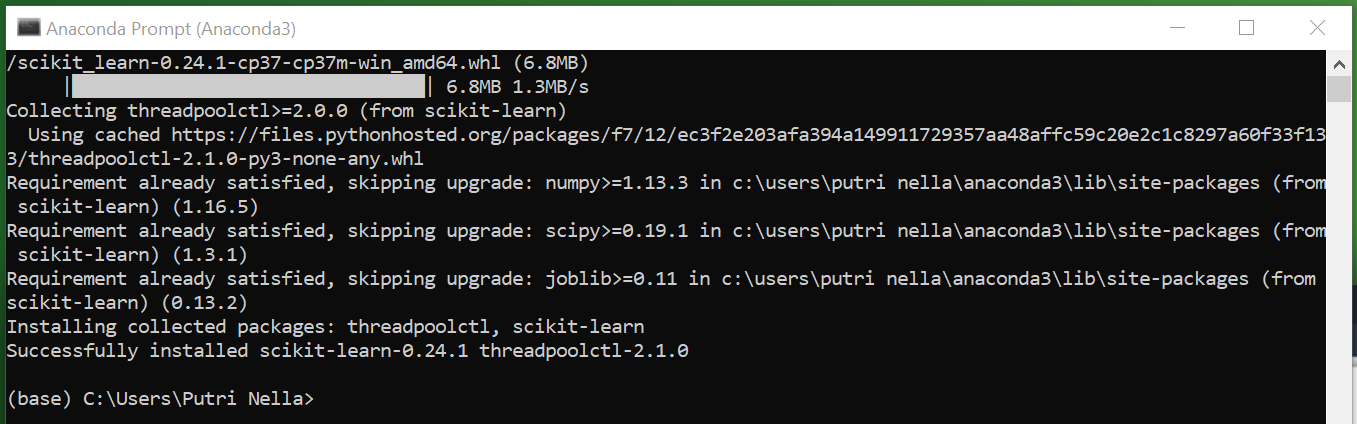
\includegraphics[width=.8\textwidth]{Pict/1.PNG}
\end{center}
    
\subsection{Example}
Untuk mengambil sebuah contoh, silahkan kunjungi website\\ https://scikit-learn.org/stable/tutorial/basic/tutorial.html lalu ambil salah satu contohnya seperti berikut ini:
\begin{lstlisting}[language=Python]
    import numpy as np
    from sklearn.model_selection import train_test_split
    from sklearn.linear_model import PoissonRegressor
    from sklearn.experimental import enable_hist_gradient_boosting 
    from sklearn.ensemble import HistGradientBoostingRegressor
    
    n_samples, n_features = 1000, 20
    rng = np.random.RandomState(0)
    X = rng.randn(n_samples, n_features)
    # positive integer target correlated with X[:, 5] with many zeros:
    y = rng.poisson(lam=np.exp(X[:, 5]) / 2)
    X_train, X_test, y_train, y_test = train_test_split(X, y, random_state=rng)
    glm = PoissonRegressor()
    gbdt = HistGradientBoostingRegressor(loss='poisson', learning_rate=.01)
    glm.fit(X_train, y_train)
    gbdt.fit(X_train, y_train)
    print(glm.score(X_test, y_test))
    print(gbdt.score(X_test, y_test))
\end{lstlisting}
Jika di running, maka akan seperti ini hasilnya:
\begin{center}
    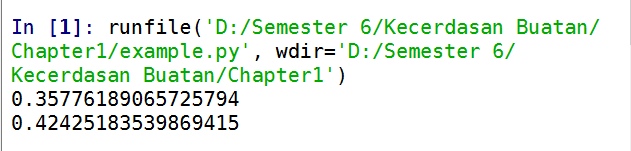
\includegraphics[width=.8\textwidth]{Pict/hasil1.PNG}
\end{center}

\subsection{Loading an example dataset}
\begin{lstlisting}[language=Python]
    from sklearn import datasets #mengimport class dataset dari scikit learn library
    iris = datasets.load_iris() #memuat dan memasukkan dataset iris ke variabel bernama iris
    digits = datasets.load_digits() #memuat dan memasukkan dataset digits ke variabel digits
    print(digits.data) #memberikan akses ke fitur yang dapat digunakan untuk mengklasifikasikan sample digit dan menampilkan di console
    digits.target #memberikan informasi tentang data yang berhubungan atau juga dapat dijadikan sebagai label
    digits.images[0] #Data selelu berupa array 2D, shape(n.samples, n.features), meskipun data aslinya mungkin memiliki bentuk yang berbeda
\end{lstlisting}
Hasilnya:
\begin{center}
    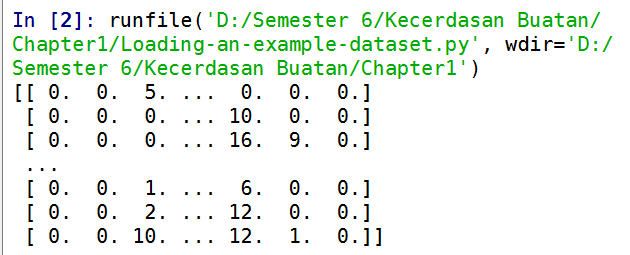
\includegraphics[width=.8\textwidth]{Pict/hasil2.PNG}
\end{center}

\subsection{Learning and predicting}
\begin{lstlisting}[language=Python]
    from sklearn import svm #perintahnuntuk mengimport class svm dari packaged sklearn
    digits = datasets.load_digits() #memuat dan memasukkan dataset digits ke variable digits
    clf = svm.SVC(gamma=0.001, C=100.) #clf sebagai estimator/parameter, svm.SVC sebagai class, gamma sebagai parameter untuk menetapkan nilai secara manual
    clf.fit(digits.data[:-1], digits.target[:-1]) #clf sebagai estimator/parameter, f i t sebagai metode, digits.data sebagai item, [:1] sebagai syntax pythonnya dan menampilkan outputannya
    print(clf.predict(digits.data[-1:])) #clf sebagai estimator/parameter, predict sebagai metode lainnya, digits.data sebagai item dan menampilkan outputannya
\end{lstlisting}
Hasilnya:
\begin{center}
    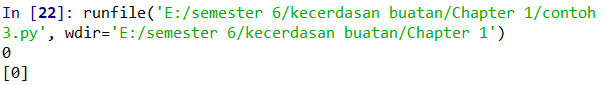
\includegraphics[width=.8\textwidth]{Pict/hasil3.PNG}
\end{center}

\subsection{Model persistence}
\begin{lstlisting}[language=Python]
    from sklearn import svm, datasets #menginport class dataset dari scikit learn library
    clf = svm.SVC(gamma=0.001, C=100.) #memanggil class SVC dan menset argumen constructor SVC serta ditampung di variabel clf
    X, y = datasets.load_iris(return_X_y=True) #meload datasets iris dan ditampung di variabel x untuk data dan y untuk target
    clf.fit(X, y) #memanggil method fit untuk melakukan training data dengan argumen data dan target dari datasets iris
    
    
    #Pickle
    import pickle
    s = pickle.dumps(clf)
    clf2 =pickle.loads(s)
    print(clf.predict(X[0:1]))
    
    #Joblib
    from joblib import dump, load
    dump(clf, '1184038.joblib')
    clf3 = load('1184038.joblib')
    print(clf3.predict(X[0:1]))
 \end{lstlisting}
 Hasilnya:
 \begin{center}
    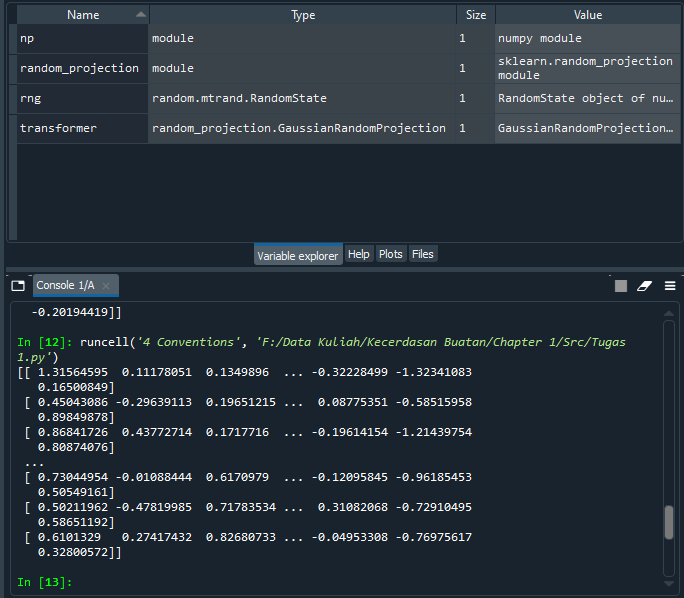
\includegraphics[width=.8\textwidth]{Pict/hasil4.PNG}
\end{center}
Selain itu, ia juga menghasilkan sebuah file joblib yang otomatis ada di dalam folder jika kita running
 \begin{center}
    
\includegraphics[width=.8\textwidth]{Pict/joblib.PNG}
\end{center}

\subsection{Conventions}
\begin{lstlisting}[language=Python]
    import numpy as np
    from sklearn import random_projection
    rng = np.random.RandomState(0)
    X = rng.rand(10, 2000)
    X = np.array(X, dtype='float32')
    print(X.dtype)
    transformer = random_projection.GaussianRandomProjection()
    X_new = transformer.fit_transform(X)
    print(X_new.dtype)
    
    from sklearn import datasets
    from sklearn.svm import SVC
    iris = datasets.load_iris()
    clf = SVC(gamma=0.001, C=100.)
    clf.fit(iris.data, iris.target)
    print(list(clf.predict(iris.data[:3])))
    clf.fit(iris.data, iris.target_names[iris.target])
    print(list(clf.predict(iris.data[:3])))

    #refiting and updatingparameter
    import numpy as np
    from sklearn.datasets import load_iris
    from sklearn.svm import SVC
    X, y = load_iris(return_X_y=True)
    clf = SVC()
    clf.set_params(kernel='linear').fit(X, y)
    print(clf.predict(X[:5]))
    clf.set_params(kernel='rbf').fit(X, y)
    print(clf.predict(X[:5]))
    
    #multiclass vc multilabel fitting
    from sklearn.svm import SVC
    from sklearn.multiclass import OneVsRestClassifier
    from sklearn.preprocessing import LabelBinarizer
    X = [[1, 2], [2, 4], [4, 5], [3, 2], [3, 1]]
    y = [0, 0, 1, 1, 2]
    classif = OneVsRestClassifier(estimator=SVC(random_state=0))
    print(classif.fit(X, y).predict(X))
    y = LabelBinarizer().fit_transform(y)
    print(classif.fit(X, y).predict(X))
    from sklearn.preprocessing import MultiLabelBinarizer
    y = [[0, 1], [0, 2], [1, 3], [0, 2, 3], [2, 4]]
    y = MultiLabelBinarizer().fit_transform(y)
    print(classif.fit(X, y).predict(X))
\end{lstlisting}
Hasilnya:
\begin{center}
    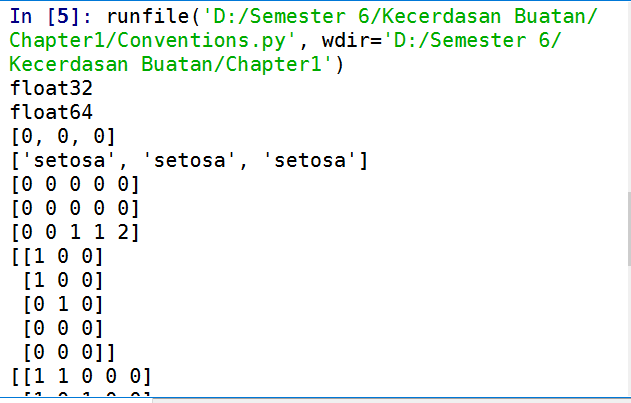
\includegraphics[width=.8\textwidth]{Pict/hasil5.PNG}
\end{center}

\section{Error}
Pada saat praktiikum, saya mengalami beberapa error, seperti:
\begin{center}
    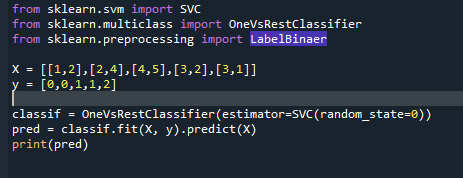
\includegraphics[width=.8\textwidth]{Pict/error1.PNG}
\end{center}
Hal ini disebabkan karena adanya variabel yang tidak dapat dipanggil. Penyelesaiannya dengan mengganti nama variabel dengan yang sudah ada dan dapat terpanggil.
\begin{center}
    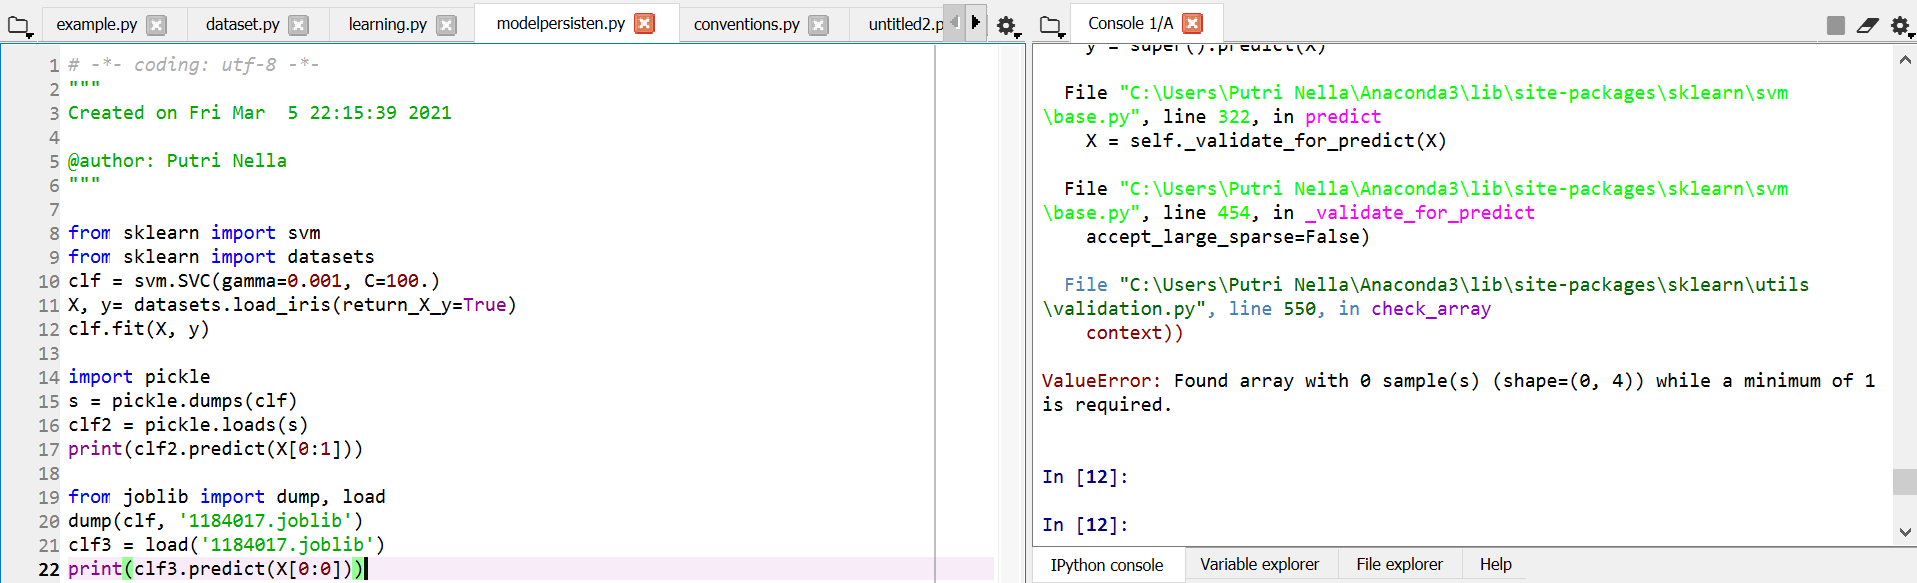
\includegraphics[width=.8\textwidth]{Pict/error2.PNG}
\end{center}
Hal ini disebabkan karena adanya kesalahan dalam penulisan kode atau tanda baca. 
\end{document}
